\documentclass[conference]{IEEEtran}

\usepackage[nolist]{acronym}
\usepackage[backend=bibtex]{biblatex}
\usepackage{graphicx}

\addbibresource{vision-transformer.bib}

\hyphenation{op-tical net-works semi-conduc-tor}


\begin{document}

  \title{\acl{vit} Architectures with Registers (Thesis outline)}

  \author{\IEEEauthorblockN{Florian Weidner}
    \IEEEauthorblockA{Philipps-University Marburg, Germany\\
      Department of Mathematics and Computer Science, Deep Learning Group\\
      February 09, 2024\\
  }}

  \maketitle
  \begin{abstract}
  The abstract goes here.
  \end{abstract}

  \begin{IEEEkeywords}
    \ac{vit}, 
    \end{IEEEkeywords}

  \IEEEpeerreviewmaketitle

  \section{Introduction}
  Introduction to the topic...

  Explanation of \acp{vit} \cite{10.1145/3505244} \cite{visiontransformers2021} \cite{vit-state-challenges} \cite{Liu2024-lm}

  \section{Vision Transformers}

  \begin{figure}
    \centering
    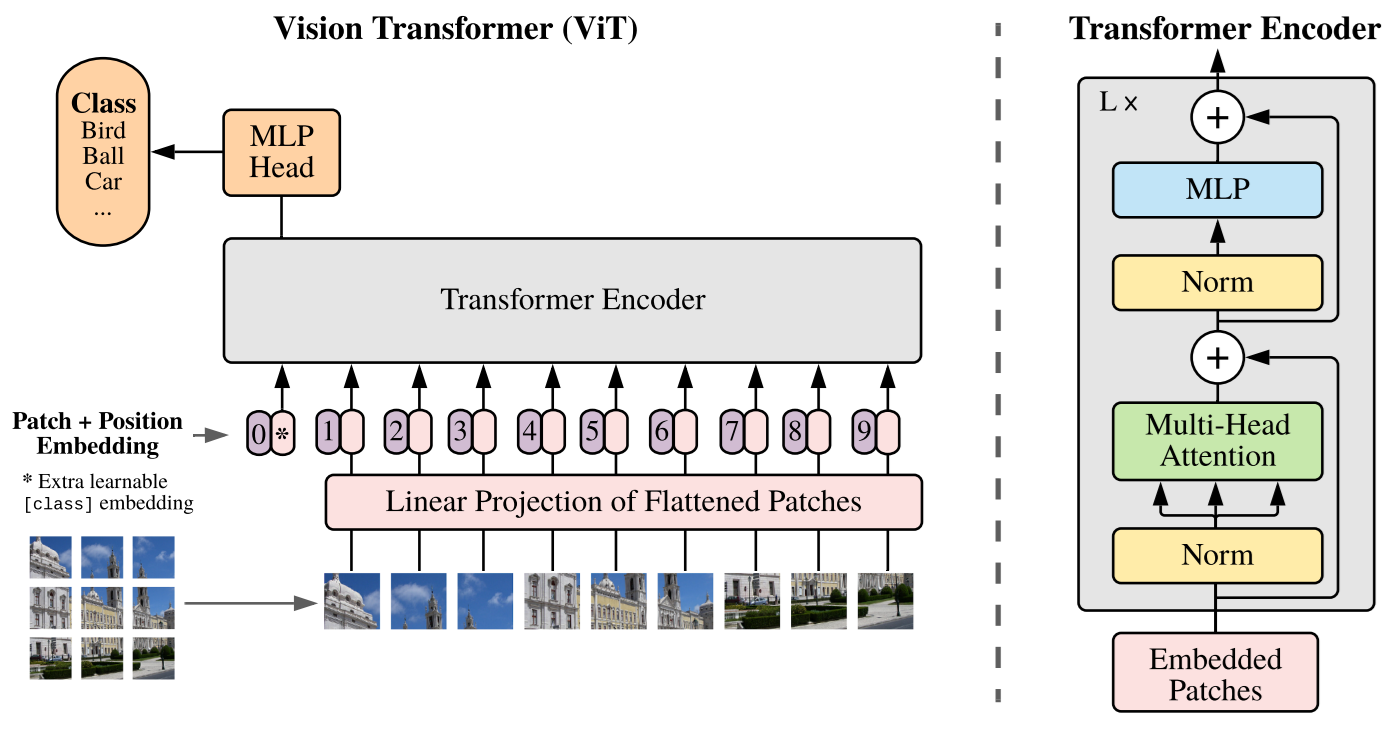
\includegraphics[width=0.5\textwidth]{figures/vit-architecture.png}
    \caption{Overview of a \ac{vit} architecture. \cite{visiontransformers2021}}
    \label{fig:vit-architecture}
  \end{figure}

  The Transformer architecture is a neural network model architecture, created primarily for sequence-to-sequence tasks in \ac{nlp}. 
  \begin{quote}
    "The key feature of transformers is the self-attention mechanism, which helps a model learn the global contexts and enables the model to acquire the long-range dependencies." \cite{vit-state-challenges}
  \end{quote}
  It consists of an encoder, which makes the input sequence into a continuos representation and a decoder, which then generates the output sequence. The encoder is built up of n identical layers, containing following components:
  \begin{itemize}
    \item multi-head self-attention mechanism: captures relationships between all tokens in the input, regardless of their distance
    \item feed-forward network: simple two-layer MLP network with ReLU activation which is applied to each token separately
    \item add \& norm layers using residual connections and layer normalization to stabilize the training
  \end{itemize}
  The result outcome of the encoder is a enriched sequence representation, which is then used by the decoder to generate the output sequence. The decoder also consits of n identical layers with:
  \begin{itemize}
    \item masked multi-head self-attention mechanism: ensures a causal generation, by preventing that tokens have impact to future tokens
    \item encoder-decoder attention mechanism: focuses on the relevant parts of the encoder's output
    \item feed-forward network: similar to the encoder
    \item add \& norm layer:ssimilar to the encoder
  \end{itemize}
  The input text is embedded and combined with a positional encoding to provide token order information. Because several attention layers can run in parallel, the architecture is significantly more parappelizable than \ac{rnn} or \ac{cnn} architectures, which makes it very efficient for modern hardware accelerators. That allows the Transformer to scale to very large models and datasets. \cite{transformer2017}

  \citeauthor{visiontransformers2021} introduced the idea of using the stated transformer architecture for computer vision. A lot of research tried to combine self-attention mechanisms with \ac{cnn} architectures, not achieving a effectively scalable method for modern hardware accelerators. \cite{visiontransformers2021} proposed to apply a standard Transformer directly to images, that are split into fixed-size patches. Each patch is flattened into a vector and passed through a linear projection layer to form an embedding as input for the Transformer. These embeddings are used as tokens in a \ac{nlp} scenario. Positional embeddings are added to retain spatial information since they process images as sequences, unlike \acp{cnn} which inherently capture spatial hierarchies. For classification tasks, an extra learnable [class] embeding is added in front of the embedded input. At the output of the encoder, the final representation of this token is used for classification. Instead of using encoder and decoder like in \ac{nlp} tasks, acp{vit} only uses the encoder since the goal is to find a better representation but an autoregressive prediciton. Additional Layer Normalization is used before the multi-head attention laver. \cite{vit-state-challenges} In figure \ref{fig:vit-architecture} you can see the architecture of a \ac{vit} including the split image patches, their embeddings combined with positional embeddings the encoder and the class embedding used for the classificaion prediction.
  \acp{vit} have much less image-specific inductive bias than \acp{cnn}, because other than \acp{cnn}, with the global self-attention mechanism spatial relationships needs to learned from scratch, but long-range dependencies across the entire image can be captured. As Transformers, \acp{vit} are normally pre-trained on large datasets and then fine-tuned to more specific tasks. After pre-training, the prediction head is removed and a zero-initialized feedforeward layer, where the size is the number of classes, is added.

  Like Transformers, \acp{vit} are also very parallelizable, which makes them very efficient. But \cite{visiontransformers2021} found out that without large-scale pre-training, \acp{vit} often underperform. So \acp{vit} requires sidnificant computational resources. But when pre-trained on large datasets, \acp{vit} outperforms \acp{cnn} on image classification tasks. The architecture performs well for transfer learning, where the pre-trained model can be fine-tuned already with limited labeled data \cite{visiontransformers2021}.  \cite{visiontransformers2021} stated that further scaling of \acp{vit} would likely lead to improved performance. Also self-supervised pre-training, where no labeled data is needed, can be improved. They found out that with mimicking the masked language modeling task used in BERT, the model performs still better than \acp{cnn} but a bit worse that with supervised pre-training of a \ac{vit}. By now different architectures and training-tricks of \acp{vit} have been proposed to further improve \acp{vit} including self-supervised learning. The architectur also got adapted for image recognition, object detection, image segmentation, pose estimation, and 3D reconstruction tasks. \cite{vit-state-challenges}

  The classical \ac{vit} architecture has been adopted and improved by many others. One approach is to include \ac{cnn} structures, which bring locality through the convolution kernels, into \acp{vit} to improve the data efficiency. DeiT \cite{deit} for example uses a \ac{cnn} as a teacher to train a \ac{vit}. It utilizes knowledge distillation of the \ac{cnn} to add the inductive bias to a vision transformer. It allows to train a \ac{vit} without the need of large-scale pre-training the model. \cite{vit-state-challenges} Another approach is to diversify the features of \acp{vit}. DeepVit \cite{deepvit} found out that the attention collapses in deeper layers, wich leads to lower performance. By adding a learnable transformation matrix after the attention layer, the model is stimulated to generate new attention maps also in the deeper layer, increasing the performance. \cite{vit-state-challenges} Also the heavy computation costs are reseached. Many also try to improve the self-supervised learning, that the pre-training with the need of large datasets can be simplified. One approach is DINO. \cite{dino} It uses a teacher-student archtecture, where the student network learns to match the avereaged outputs of the teacher. \cite{vit-state-challenges} The following summerized paper, identifies and addresses artifacts in attention maps of supervised and self-supervised \ac{vit} networks.

  \cite{deit3} \cite{open-clip}

  \section{Vision Transformers need registers: A summary}

  In this chapter we summerize the paper \cite{registers}. The paper discoverd artifacts and proposes to use additional register tokens for \acp{vit} to remove these artifacts.

  \subsection{Artifacts in Vision Transformers}
  \begin{figure}
    \centering
    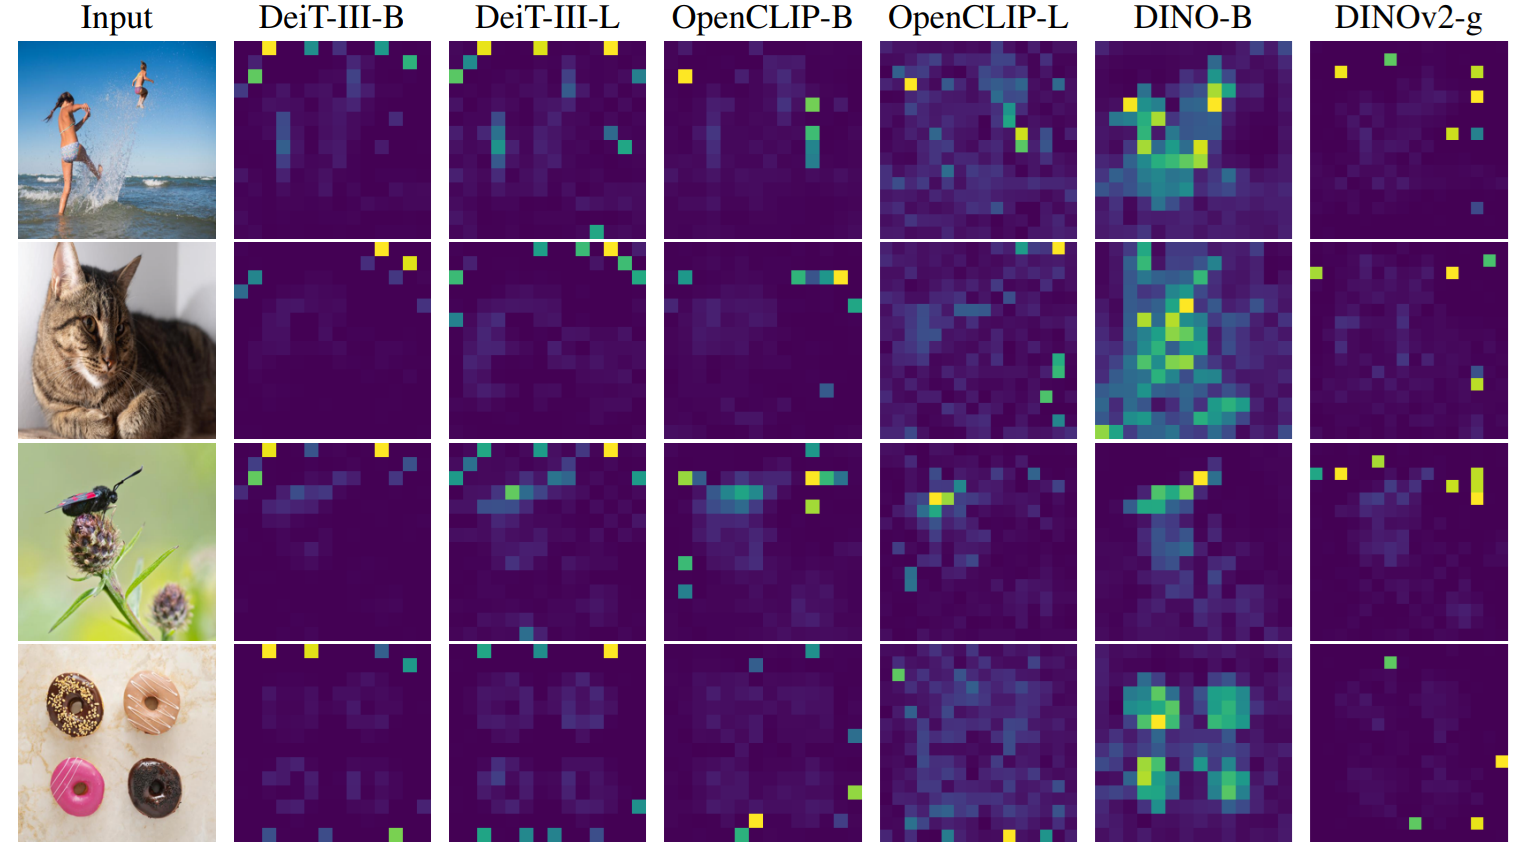
\includegraphics[width=0.5\textwidth]{figures/vits-artifacts.png}
    \caption{Illustration of artifacts observed in the attention maps of modern vision transformers. \cite{registers}}
    \label{fig:artifacts-observations}
  \end{figure}


  After introducing to \acp{vit} like we did in this paper, the models they found the artifacts are introduced. The DINO algorithm is a self-supervised learning method, that uses two \acp{vit}. A student network is predicting the output of a teacher network, to learn rich representaions of visual data without the need of manual annotations. \cite{dino} DINO is shown to produce models, that contain semantically consistent information in the last attention layer. Object discovery algorihtms like LOST \cite{lost}, built on top of DINO, are using these attention maps, that often contains semantically interpretable information, used to detect objects without supervision. DINOv2 \cite{dinov2} is a improved followup focusing on dense predition tasks, which are tasks, where detailed outputs are required to provide fine-grained localized informations, like semantic segementation or depth estimation. Despite good performance on these dense tasks, the authors observed that DINOv2 is incompatible with LOST \cite{registers}. The different behaviour of DINO and DINOv2 can be observed in the artifacts in the last attention maps. In figure \ref{fig:artifacts-observations} you can see the different models and their artifacts on the last attention layer.
  While DINO shows no peak outlier values focusing the main object in the image, DINOv2 shows a lot of artifacts on the background of the images. This qualitatively observation can be also made for the label-supervised model DeiT-III and the text-supervised model OpenCLIP. Shown in figure \ref{fig:artifacts-observations}, you can observe similar artifacts in the background.
  To explain why and where the artifacts of \acp{vit} in attention maps appear, the paper focuses on DINOv2. 

  Artifact patches show higher norm of their token embedding at the output of the model than other patches. In figure \ref{fig:artifacts-norm} you can see the distribution of the local feature norms over a small dataset. While for DINO, the norm stays under 100 for all patches, DINOv2 shows a lot of patches with a norm higher than 150. This cutoff value can vary across different models. They define artifacts as
  \begin{quote}
    "tokens with norm higher than 150 will be considered as “high-norm” tokens" \cite{registers}
  \end{quote}

  The authors found different conditions, when the artifacts appear in the training process of DINOv2. Figure \ref{fig:artifacts-layer} shows the following conditions:
  \begin{itemize}
    \item artifacts start appearing around layer 15 to 40.
    \item artifacts start appearing after on thrid of training.
    \item artifacts only appear in the three largest model versions
  \end{itemize}

  \begin{figure}
    \centering
    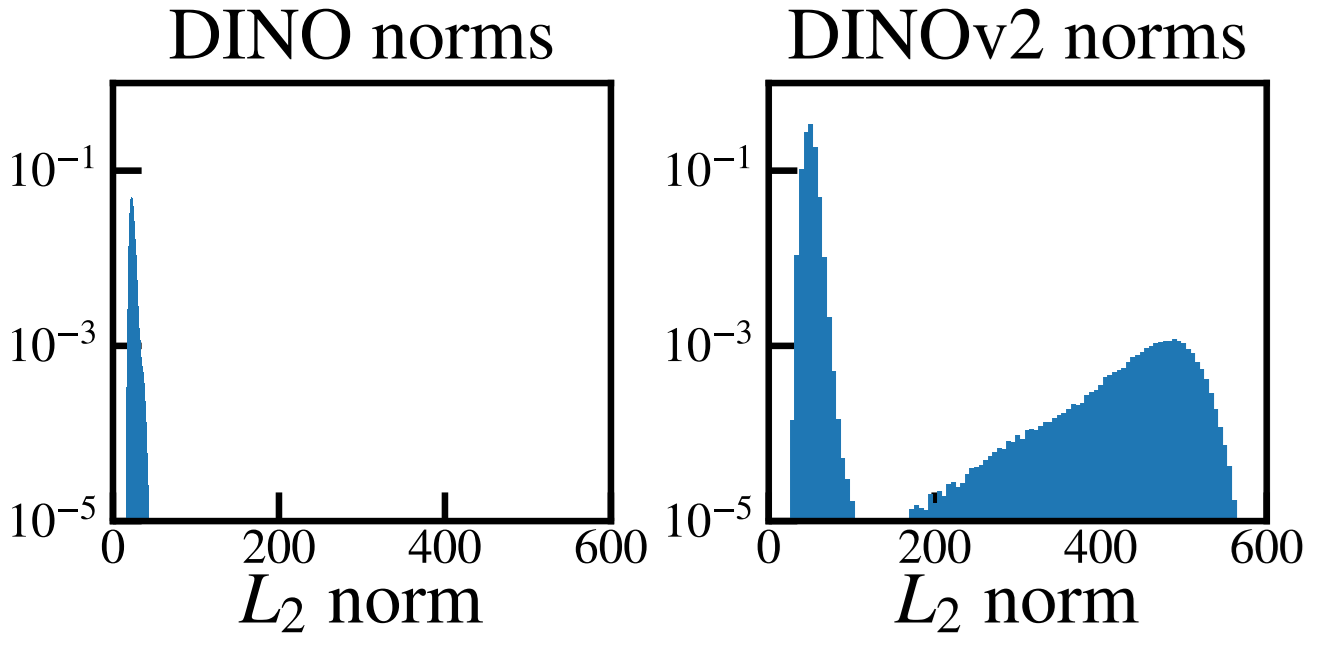
\includegraphics[width=0.3\textwidth]{figures/artifact-norm.png}
    \caption{Comparison of local feature norms for DINO ViT-B/16 and DINOv2 \cite{registers}}
    \label{fig:artifacts-norm}
  \end{figure}
  \begin{figure}
    \centering
    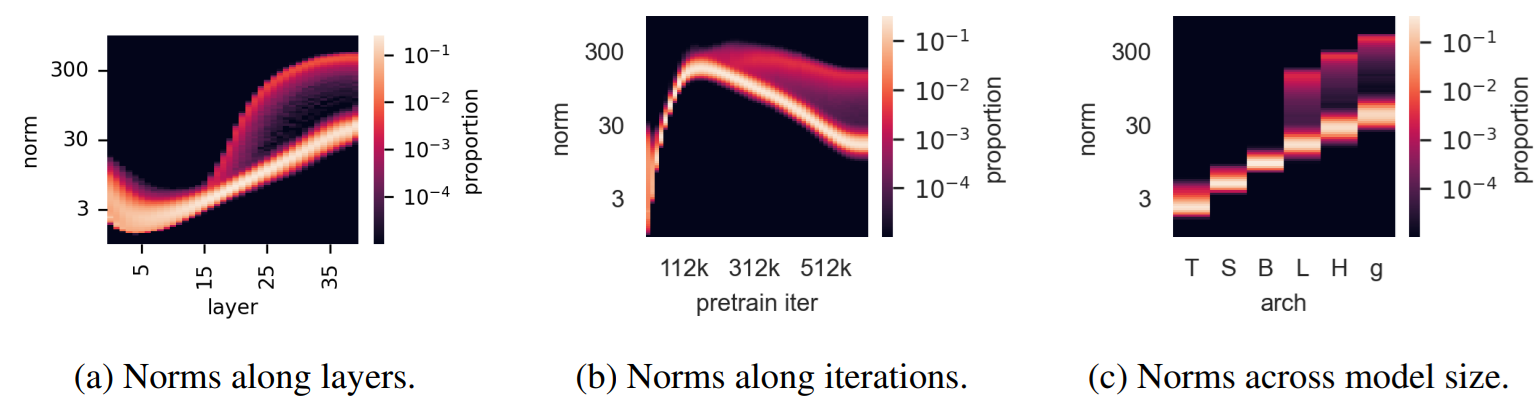
\includegraphics[width=0.5\textwidth]{figures/artifact-layers.png}
    \caption{Illustration of several properties of outlier tokens in the 40-layer DINOv2 ViT-g model \cite{registers}}
    \label{fig:artifacts-layer}
  \end{figure}

  Another discovery is that the high-norm tokens appear where patch information is redundant. The authors tested the cosine similarity between high-norm tokens and their four neighbors, directly after the image is emebdded. They observed, that the high norm patches appear where their cosine similarity to the neighbors is high. Compared to the observations, that shows that artifacts appear mostly in the background of images, high-norm pathes seem to have redundant information, that the model can ignore, to achive similar scores at the output.

  To further understand the outlier tokens, two linear models were trained, to check the embeddings for different information. Both models were trained on the patch embeddings, the embeddings of the images (see figure \ref{fig:vit-architecture}). The result performance is compared between using high-norm tokens and normal tokens. The first task was position prediction. The model should predict the position of a patch token in the image and measure the accuracy. They observed that high-norm tokens have much lower accuracy than the other tokens and suggested that they contain less information about the position in the image. The second task was pixel reconstruction. The model should predict the pixel value of an image from the patch embeddings and mesaure the accuracy of this model. Also here the high-norm tokens have  lower accuracy than the other tokens. The authors concluded that the high-norm tokens contain less information to reconstruct the image than the others. 
  The authors also found out that the high-norm tokens hold more global information by training a logistic regression model. The model predicts the image class by the patch embedding of a random token. I turned out that the high-norm tokens have a much higher accuracy than the other tokens. This suggests that the high-norm tokens contain more global information about the image than the other tokens. 

  Making these obervations the authors make following hypsthesis:
  \begin{quote}
    "Large, sufficiently trained models learn to recognize redundant tokens, and to use them as places to store, process and retrieve global information." \cite{registers}
  \end{quote}

  \subsection{Registers for Vision Transformers}


  To address the behaviour, the use of registers is proposed. Since the high-norm patches are overtaking local patch information, even they are mostly not important, it possibly decreases the performance on dense prediction tasks. The called registers are additional tokens after the patch embeddings of the images with a learnable value. They work similar to the [class] token, used for classificaion tasks. They are used durning training and inference and they are discarded afterwards. In figure \ref{fig:register-architecture} you can see the register tokens additionally used after the embedding of the image. A complexity analysis show that adding registers increase the FLOPs by up to 6\% for 16 registers. With four registers, that are more commonly used, the increase is below 2\%.

  \begin{figure}
    \centering
    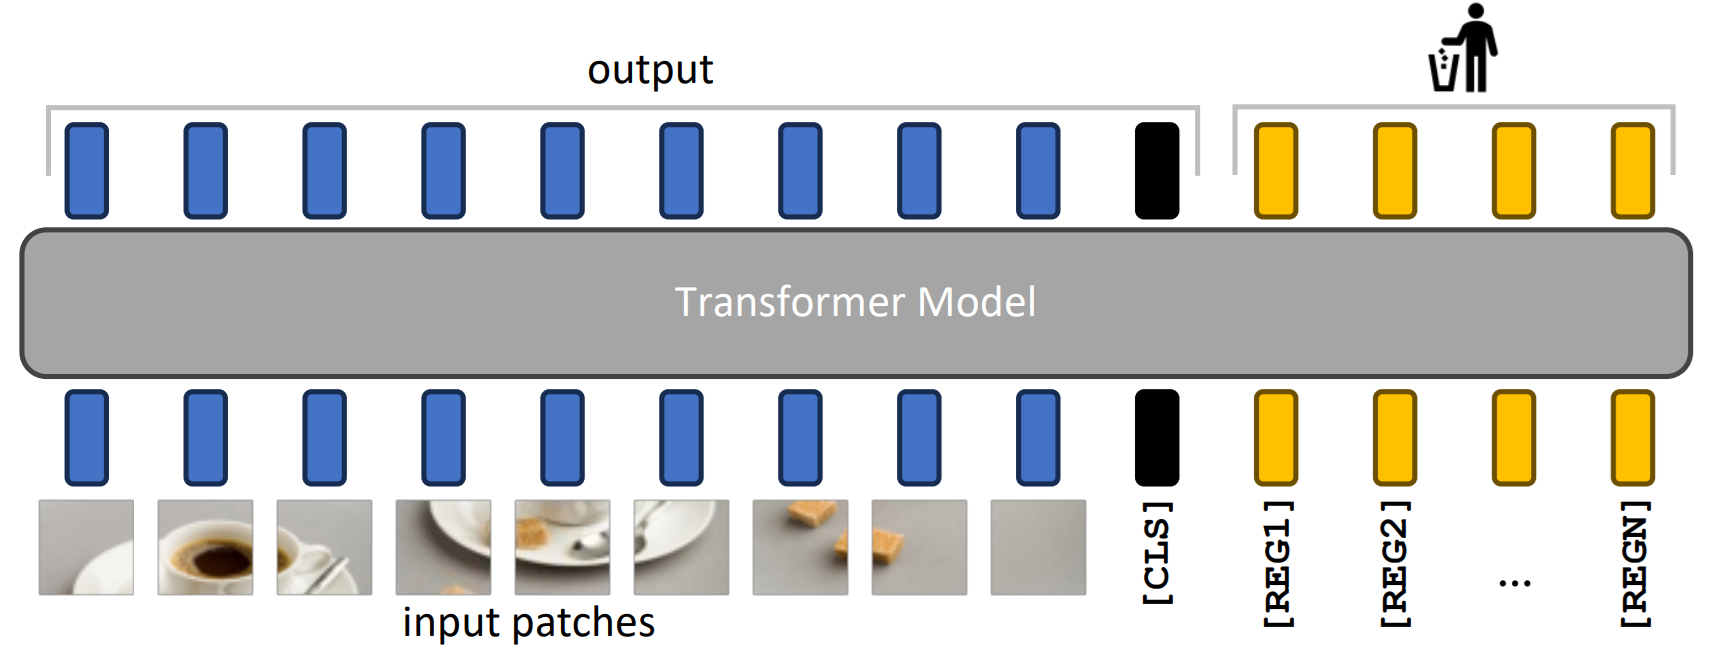
\includegraphics[width=0.5\textwidth]{figures/register-architecture.png}
    \caption{Illustration of the proposed remediation and resulting model \cite{registers}}
    \label{fig:register-architecture}
  \end{figure}

  \subsection{Evaluation of the proposed architecture}

  In the last part of the paper they validate their architecture by training \acp{vit} with register tokens and compare them  quantitativly and qualitativly to the models without token registers. They are evaluating for DEIT-III, OpenCLIP and DINOv2 architectures, therfore including label-supervised, text-supervised and self-supervised learning approaches. In figure \ref{fig:register-result} you can see three example images including attention maps with and without the use of register tokens. Qualitativly, for all three models, the artifacts in the attention maps are gone. They mesaured quantitativly the effect by calculating the norm of the attention maps at the output of the model. In figure \ref{fig:register-norm-result} you can see the distribution of the output norms for the three models. For all three models, training it with register tokens removes high-norm tokens, that were present without the token registers. Instead the attention maps of the register tokens have  higher norm than the patch and the class tokens. The register tokens are adapting the behaviour of the outlier patches of the model without registers. Visualizations are also showing that the attention maps of the register tokens look similar to the attention maps of the class tokens, all showing a larger support area. The attention maps of the patch tokens are more localized. Since the class token carries global informations, it suggests that the register tokens are also used to store global information. 
  Comparing the performance of the models with and without register tokens, linear probing on ImageNet classification, ADE20k Segmentation, and NYUd monocular depth estimation datasets was used. The results show no lose in performance, when additoinally using register tokens. Also for zero-shot classification on ImageNet with OpenCLIP, the performance is not affected by using register tokens. They also found out that one register is enough to remove the high-norm tokens in the attention maps. For DINOv2 and DeiT-III, adding register tokens significantly improves the discovery performance and for OpenCLIP, the performance is slighty worse with registers. They concluded that their proposal improves the performance in dense prediction and object discovery.

  \begin{figure}
    \centering
    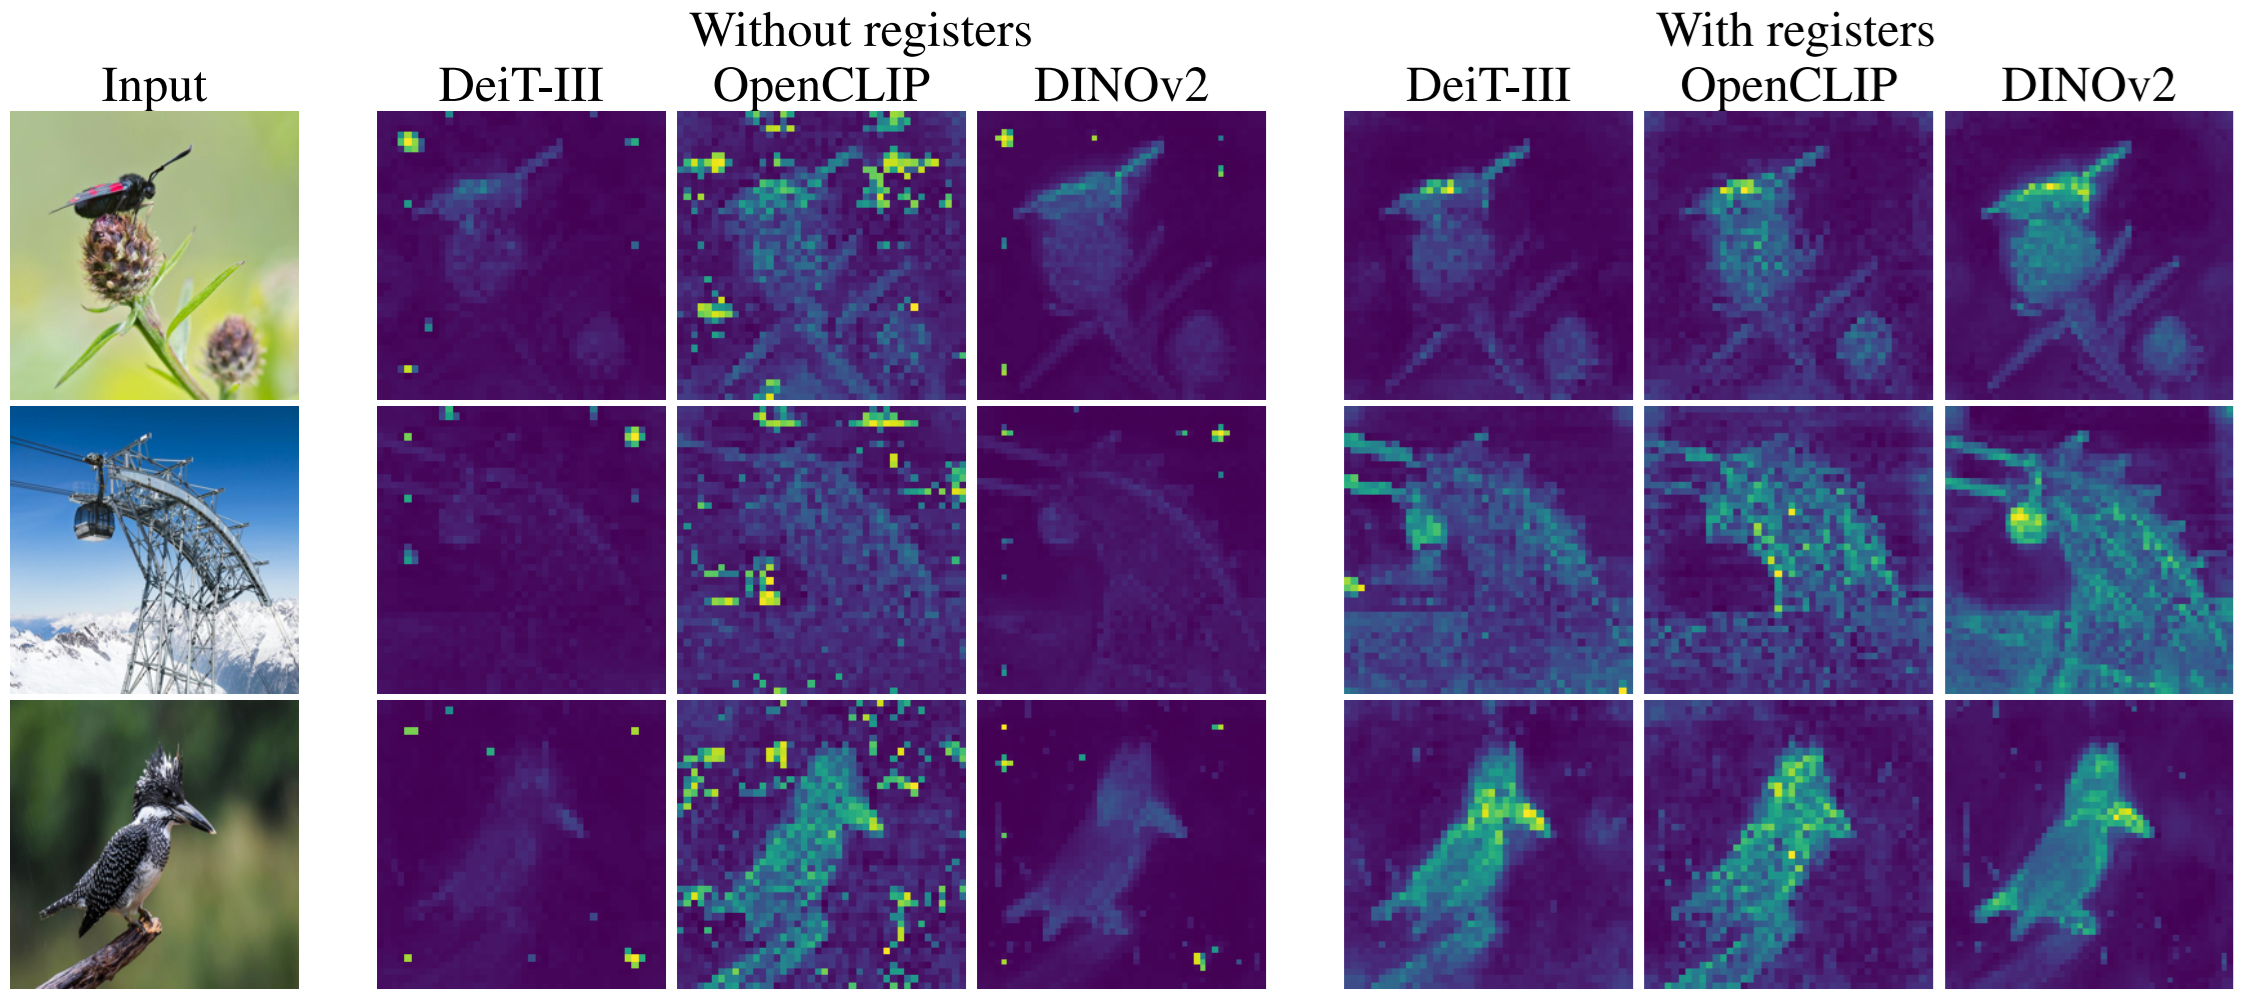
\includegraphics[width=0.5\textwidth]{figures/register-result.png}
    \caption{Three examples of attention maps with and without register tokens \cite{registers}}
    \label{fig:register-result}
  \end{figure}

  \begin{figure}
    \centering
    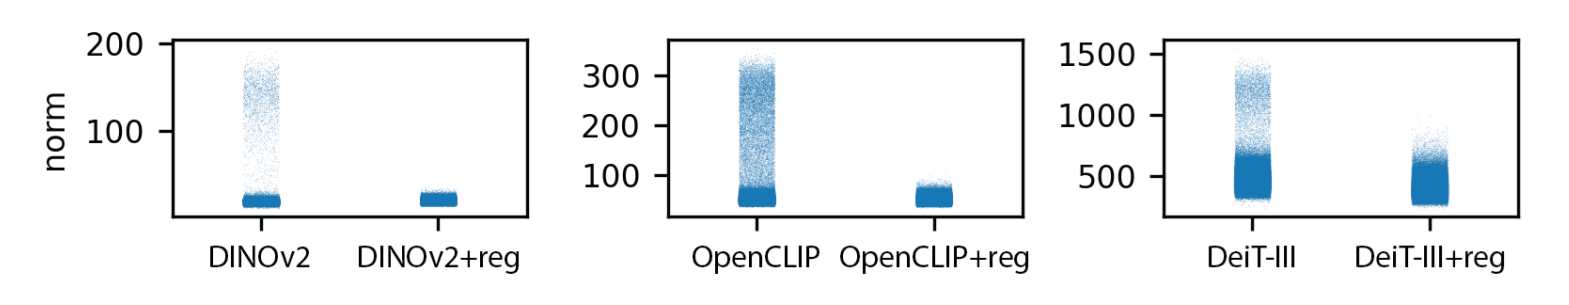
\includegraphics[width=0.5\textwidth]{figures/register-norm-result.png}
    \caption{: Effect of register tokens on the distribution of output norms \cite{registers}}
    \label{fig:register-norm-result}
  \end{figure}


  \section{Comparison to other papers with performance improvements of \ac{vit}s}

  \subsection{\cite{mamba-needs-registers} applies the idea of registers to a \ac{ssm}}

  \subsection{\cite{sum-tokens-to-registers} uses a token learner to improve the performance of \ac{vit}s}

  \subsection{\cite{token-learner} also uses a token learner to improve the performance of \ac{vit}s}


  \section{Conclusion}
  The conclusion goes here.

  \printbibliography

  \begin{acronym}
    \acro{vit}[ViT]{Vision Transformer}
    \acroplural{vit}[ViTs]{\ac{vit}s}
    \acro{nlp}[NLP]{Natural Language Processing}
    \acro{cnn}[CNN]{Convolutional Neural Network}
    \acroplural{cnn}[CNNs]{\acp{cnn}}
    \acro{rnn}[RNN]{Recurrent Neural Network}
    \acro{mlp}[MLP]{Multi-Layer Perceptron}
    \acro{ssm}[SSM]{n State Space Model}
  \end{acronym}


that's all folks
\end{document}


